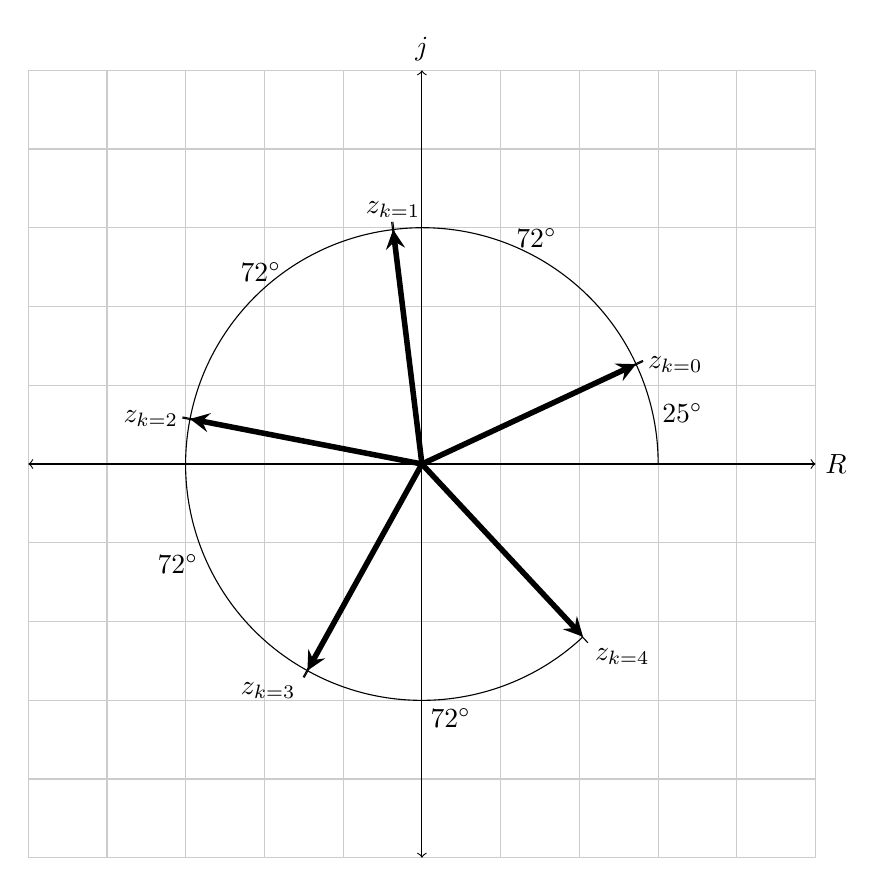
\begin{tikzpicture}
        \draw[thin,gray!40] (-5,-5) grid (5,5);
        \draw[<->] (-5,0)--(5,0) node[right] {$R$};
        \draw[<->] (0,-5)--(0,5) node[above]{$j$};
        \draw[line width=2pt,black,-stealth](0,0)--(2.72,1.268) node[right]{${z_{k=0}}$};
        \draw[line width=2pt,black,-stealth](0,0)--(-0.3656,2.977) node[above]{${z_{k=1}}$};
        \draw[line width=2pt,black,-stealth](0,0)--(-2.945,0.5724) node[left]{${z_{k=2}}$};
        \draw[line width=2pt,black,-stealth](0,0)--(-1.4544,-2.624) node[anchor=north east]{${z_{k=3}}$};
        \draw[line width=2pt,black,-stealth](0,0)--(2.046,-2.194) node[anchor=north west]{${z_{k=4}}$};
        \draw[|-|] (3,0) arc (0:25:3) node [midway, right]{$25^{\circ}$};
        \draw[|-|] (2.72,1.268) arc (25:97:3) node [midway,above]{$72^{\circ}$};
        \draw[|-|] (-0.3656,2.977) arc (97:169:3) node [midway, above]{$72^{\circ}$};
        \draw[|-|] (-2.945,0.5724) arc (169:241:3) node [midway, left]{$72^{\circ}$};
        \draw[|-|] (-1.4544,-2.624) arc (241:313:3) node [midway, below]{$72^{\circ}$};
    \end{tikzpicture}
    \caption{Representación de la ecuación \ref{eq:RadCej} en el intervalo marcado}